\section{CHAPTER 7: BOILERS}
\subsection{Acquaintance}
Boilers represent critical equipment in todays industrial proceses and home heating setups, converting water into steam or heated water through different fuel types like natural gas, oil, coal, or electrical power. The thermal energy produced are then used for heating purposes, power production, and various other uses. Starting from basic fire-tube concepts to modern water-tube and electric configurations, boilers has become essential across different sectors, such as manufacturing, power generation, and food industries. There importance stems from delivering steady and dependable heat and steam, which are crucial for many industrial operations. Contemporary boilers were designed with enhanced efficiency, environmental considerations, and safety features, incorporating technology such as condensing systems too recover exhaust heat and advanced control mechanisms for optimal functioning and safety protocols. Knowledge regarding various boiler types, there components, and operational principals is essential for personnel involved in maintenance, operations, or engineering. This report examine the various boiler classifications, operational mechanisms, and recent technological developments, emphasizing there vital role in modern industry and everyday applications.
\begin{figure}[h]
\centering
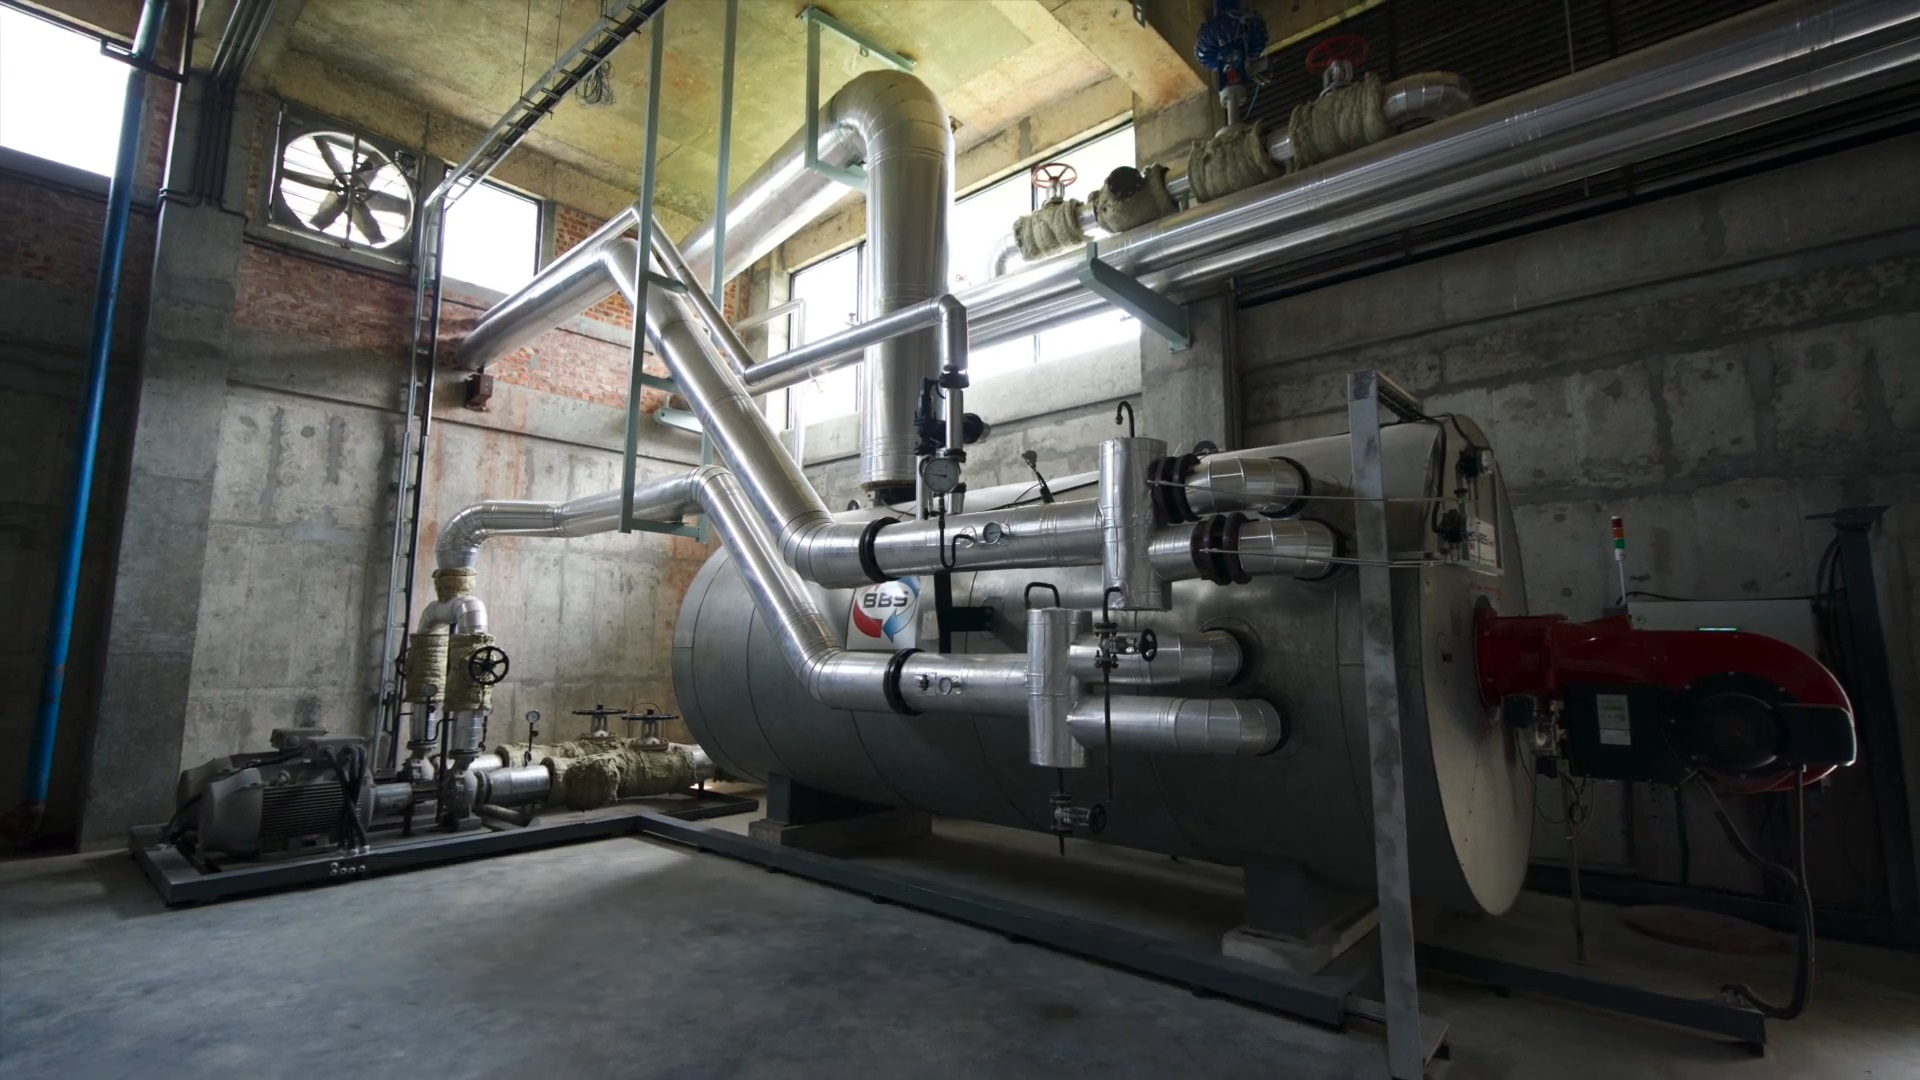
\includegraphics[width=0.8\textwidth]{figs/boiler.jpg}
\caption{Boiler}
\label{fig:boiler}
\end{figure}


\subsection{Types of Boilers \cite{steam_boilers}}
Boilers could be categorised into different types based on various criterias. Following is an detailed overview of main types:

\subsubsection{Based on the position of water and hot gases}
\begin{enumerate}
    \item \textbf{Fire Tube Boiler}: Heated gas move inside tubes while water surrounds em.
    \item \textbf{Water Tube Boiler}: Water moves in tubes while hot gas heat from outside.
\end{enumerate}

\subsubsection{Based on the position}
\begin{enumerate}
    \item \textbf{External Fired Boiler}: The furnace assembly remains separate from the main shell.
    \item \textbf{Internally Fired Boiler}: Contains furnace integrated within the shell structure.
\end{enumerate}

\subsubsection{Based on Axis}
\begin{enumerate}
    \item \textbf{Horizontal Boiler}: These type have horizontal axis orientation.
    \item \textbf{Vertical Boiler}: Such boilers are having vertical axis alignment.
\end{enumerate}

\subsubsection{Based on Pressure}
\begin{enumerate}
    \item \textbf{Low-Pressure Boiler}: Functions at pressure lesser than 15 psi.
    \item \textbf{High-Pressure Boiler}: Operations occur above 15 psi pressure.
\end{enumerate}

\subsubsection{Based on the Furnace}
\begin{enumerate}
    \item \textbf{Single Furnace Boiler}: Has got one furnace unit.
    \item \textbf{Dual Furnace Boiler}: Equipped with two furnace units.
\end{enumerate}

\subsubsection{Based on the Method of Circulation}
\begin{enumerate}
    \item \textbf{Natural Circulation Boiler}: Waters circulate naturally due too convection current.
    \item \textbf{Forced Circulation Boiler}: Water movement is achieved through pump.
\end{enumerate}

\subsubsection{Based on Fuel Burning}
\begin{enumerate}
    \item \textbf{Solid Fuel-Fired Boiler}: This functions with solid materials such as wood or coal.
    \item \textbf{Oil and Gas Fired Boiler}: It is designed to operate with both oil and gas inputs.
    \item \textbf{Dual Fired Boiler}: Can operate with both oil and gas.
    \item \textbf{Exhaust Gas Boiler}: Mainly uses waste heat from exhaust gases, making them unique in terms of fuel usage.
\end{enumerate}

\subsubsection{Based on the Furnace}
\begin{enumerate}
    \item \textbf{Single Furnace Boiler}: Comprises one furnace.
    \item \textbf{Dual Furnace Boiler}: Incorporates two furnaces.
\end{enumerate}


\textbf{Fire-tube Boilers:}
These systems work by directing combustion gases through submerged tubes surrounded by water. Heat transfer occurs between hot gases and water, producing steam for various uses. The simple yet robust design makes these units reliable for different heating needs, particularly in smaller operations.

\textbf{Water-Tube Boilers:}
Unlike fire-tubes, these units channel water inside tubes while hot gases flow around them. Such an arrangement delivers better thermal efficiency and allows operation at increased pressure levels. Most power plants prefer this design due to its superior performance characteristics in large-scale operations.

\textbf{Electric Boilers:}
Rather than burning fuel, these units convert electrical energy into heat. Resistance elements handle the heating process, creating a compact solution that needs minimal installation space. Commonly found where traditional fuel sources prove impractical, especially in modern building setups.

\textbf{Combi Boilers:}
These dual-purpose units handle both space heating and water heating tasks simultaneously. Their popularity stems from eliminating separate water heaters while providing instant hot water access. Residential installations frequently choose this option because it saves space and simplifies system maintenance.
\begin{figure}[h]
\centering
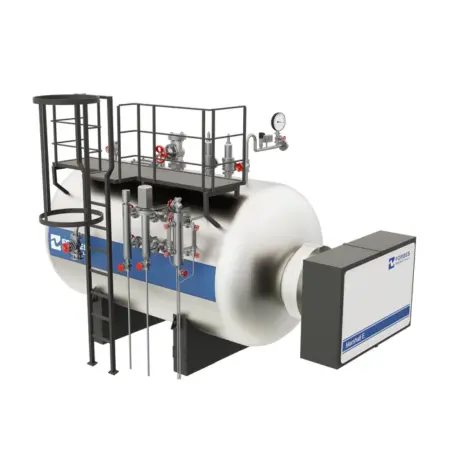
\includegraphics[width=0.45\textwidth]{figs/lastmin/electric_steam_boiler.png}
\caption{Electric Boiler}
\label{fig:Electric Boiler}
\end{figure}

\subsection{Components of a Boiler}
A boiler system contains numerous essential parts that work together ensuring safe and efficient operation. Here's a breakdown of these critical components:

\begin{figure}[h]
\centering
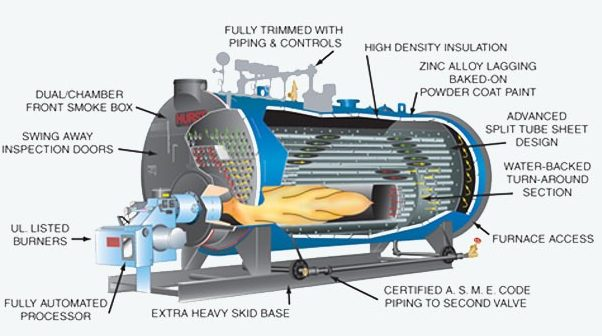
\includegraphics[width=0.8\textwidth]{figs/lastmin/boiler_components.png}
\caption{Components of a Boiler}
\label{fig:boiler_components}
\end{figure}

\begin{enumerate}
    \item \textbf{Furnace Tube}\\
    Acts as primary combustion zone where fuel burns to generate required heat energy.

    \item \textbf{Tubes (2nd Pass)}\\
    Secondary pathway for hot gases, extracting additional heat while gases move through system.

    \item \textbf{Tubes (3rd Pass)}\\
    Final heat extraction pathway, maximizing thermal efficiency through extended gas travel.

    \item \textbf{Combustion Chamber}\\
    Main burning area that holds fuel-air mixture during combustion process. Contains special materials and design features for optimal heat distribution.

    \item \textbf{Front Smoke Box}\\
    Gathers exhaust gases at forward section, guiding them toward heat exchange areas.

    \item \textbf{Rear Outlet Box}\\
    Manages exhaust gas collection at back end, directing them toward final exit point.

    \item \textbf{Sight Glass}\\
    Transparent section letting operators check water levels without stopping operation.

    \item \textbf{Safety Valve}\\
    Pressure relief mechanism that activates when system exceeds safe limits.

    \item \textbf{Crown Valve}\\
    Top-mounted steam control valve managing high-pressure steam release.

    \item \textbf{Feed Check Valve}\\
    Controls water input while preventing reverse flow, maintaining proper water balance.

    \item \textbf{Level Controls \cite{level_control}}\\ 
    Monitors and adjusts water quantity, protecting system from running dry.

    \item \textbf{Manhole}\\
    Service entry point allowing maintenance crew access for internal checks.

    \item \textbf{Spare}\\
    Additional connection point kept available for future system modifications.

    \item \textbf{Feed Pump}\\
    Maintains steady water supply ensuring continuous operation cycles.

    \item \textbf{Control Panel}\\
    Central command station housing various monitoring and adjustment tools.

    \item \textbf{Burner}\\
    Primary heat generator mixing fuel with air for controlled combustion. Features precise controls for optimal fuel usage and clean burning.

    \item \textbf{FD Fan (Forced Draft Fan)}\\
    Supplies necessary air volume maintaining proper combustion conditions.

    \item \textbf{Fan Inlet Silencer}\\
    Noise reduction device fitted to intake area reducing operational sound levels.
\end{enumerate}

\subsubsection{Combustion Chamber}
A combustion chamber serves as vital space within boiler systems where fuel-air mixtures undergo burning processes to generate thermal energy. Various configurations exist for these chambers, which could take forms such as cylindrical, rectangular, or conical shapes, depending upon specific applications and requirements of the boiler system.

\textbf{Key Aspects of the Combustion Chamber:}
\begin{enumerate}
    \item \textbf{Shape and Design:} Configuration choices affect both combustion quality and heat transfer capabilities. Industrial applications commonly utilize cylindrical designs due to there superior pressure resistance characteristics. Larger utility installations might implement rectangular configurations to accomodate expanded heat transfer surface area.
    \item \textbf{Refractory Materials:} Heat-resistant components line chamber walls, consisting materials like firebrick, castable refractories, and ceramic fiber compositions. These materials serve dual purposes - protecting outer boiler components while reflecting thermal energy back into combustion zones, thereby enhancing system efficency.
    \item \textbf{Baffles and Flame Holders:} Such components create turbulent conditions within chamber environments. Enhanced mixing between fuel and air results from these installations, leading towards complete combustion processes. Additional benefits include improved flame stability characteristics within operational parameters.
    \item \textbf{Burner Mounting:} Burner placement facilitates fuel introduction and mixing operations. Precise positional considerations ensure optimal fuel distribution patterns and maintain stable flame conditions, which directly impacts heat generation efficiency.
    \item \textbf{Heat Transfer Optimization:} Chamber designs incorporate features maximising thermal energy transfer toward heat exchanger surfaces. Careful consideration of design elements ensures efficient energy absorption by water or steam mediums, thus improving system performance metrics.
    \item \textbf{Combustion Air Supply:} Preheated air delivery systems support complete combustion processes. Such arrangements minimize energy losses while maintaining stable flame characteristics throughout operational cycles.
    \item \textbf{Exhaust Gas Path:} Post-combustion gases require efficient removal through designated pathways. These routes typically terminate at flue or chimney structures, ensuring proper gas expulsion. Careful consideration of exhaust path design elements contributes towards minimizing thermal losses and maintaining optimal system efficiency.
\end{enumerate}

\subsubsection{Heat Exchanger}
Heat exchangers serve as vital parts in boiler systems, handling thermal transfer between hot gases and water/steam. Their build quality and design directly affects how well the whole system performs.
\begin{figure}[h]
\centering
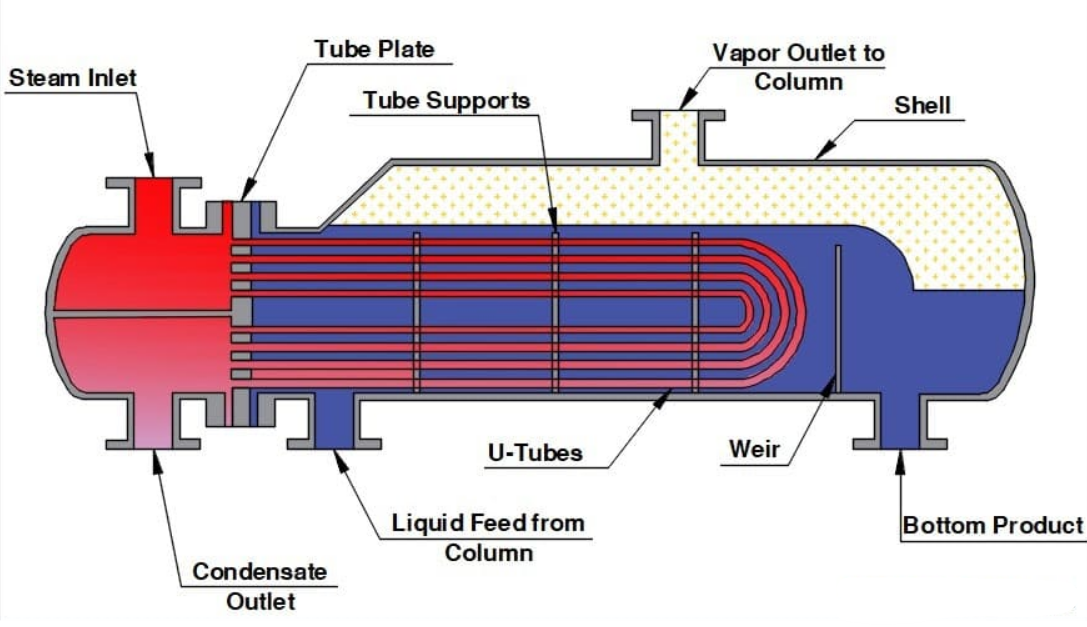
\includegraphics[width=0.8\textwidth]{figs/lastmin/heat_exchanger.png}
\caption{Heat Exchanger}
\label{fig:heat_exchanger}
\end{figure}
Key Aspects of the Heat Exchanger:
\begin{enumerate}
    \item \textbf{Function:} Works as thermal transfer station, boosting water or steam temperature levels. Without this process, boilers couldn't deliver the heating output needed for different uses.
    \item \textbf{Construction:} Most units use tough metals like steel or cast iron, picked for heat conducting abilities and long service life. The structure contains multiple passages - some designs put hot gases inside tubes while others run water through them, depending on boiler type.
    \item \textbf{Heat Transfer Mechanism:} Energy moves through two main ways - conduction thru metal surfaces and convection from fluid movement. Hot gases passing near tube walls transfer heat into the metal, which then passes to water or steam. Natural movement of fluids helps spread heat more evenly throughout system.
    \item \textbf{Water or Fluid Circulation:} Design varies based on type - fire-tube models keep water around tubes while water-tube versions run it inside them. Some systems use pumps for circulation, others rely on natural heat movement patterns.
    \item \textbf{Efficiency Considerations:} Performance depends heavily on exchanger condition. Regular cleaning and proper maintenance prevents buildup that could block heat flow. Good water treatment helps avoid scale formation, keeping system running at peak efficiency.
    \item \textbf{Combustion Gas Exhaust:} After heat extraction, waste gases leave through exhaust systems. Modern condensing 
\end{enumerate}

\subsubsection{Water Vessel}
Often called boiler shell, this sealed container holds water and steam while managing heat exchange processes. Think of it as the main chamber where all critical operations happen.
Key Features:
\begin{enumerate}
    \item \textbf{Pressure Containment:} Built tough enough to handle intense internal forces during operation. Special design prevents any unwanted steam escape or structural problems.
    \item \textbf{Heat Transfer Surface:} Inner walls maximize thermal exchange between hot gases and water. Smart surface engineering helps squeeze out better performance.
    \item \textbf{Material:} Uses premium-grade steel or special alloys that stand up to extreme heat and pressure conditions over long service periods.
\end{enumerate}

\subsubsection{Pressure Vessel}
Works as primary containment system for managing high-pressure conditions inside boiler setup. Keeps everything running smooth while maintaining safe operating environment.
Essential Elements:
\begin{enumerate}
    \item \textbf{Design Standards:} Follows strict manufacturing rules set by industry experts. Every aspect meets or exceeds safety requirements for pressure equipment.
    \item \textbf{Safety Features:} Comes equipped with pressure release mechanisms and multiple backup systems. These prevent dangerous pressure buildup during operation.
\end{enumerate}

\subsubsection{Controls and Safety Devices}
Modern boilers rely on sophisticated control systems and safety mechanisms that work together keeping operations within safe parameters while maintaining peak performance.
Key System Elements:

\begin{enumerate}
    \item \textbf{Pressure Switches:} Keep watch over internal pressure levels, triggering responses when limits approach danger zones.
    \item \textbf{Temperature Sensors:} Monitor heat conditions throughout system, helping maintain ideal operating ranges.
    \item \textbf{Safety Valves:} Act as pressure relief points, automatically releasing excess pressure before dangerous levels build up.
    \item \textbf{Flame Safeguards:} Watch over combustion process, cutting fuel supply if flame disappears unexpectedly.
    \item \textbf{Control Panels:} Serve as command center where operators manage settings and monitor system status through integrated displays.
\end{enumerate}

\subsubsection{Pumps}
Different pump types handle specific tasks keeping fluid moving properly throughout boiler system.
Critical Pump Functions:
\begin{enumerate}
    \item \textbf{Feedwater Pumps:} Handle fresh water delivery into system, maintaining proper levels for continuous operation.
    \item \textbf{Circulation Pumps:} Move water through heating zones, ensuring efficient heat distribution across system.
    \item \textbf{Condensate Pumps:} Collect and redirect condensed steam back into main water supply loop.
\end{enumerate}

\subsubsection{Expansion Tank}
Functions as pressure management system, giving water space to expand or shrink during temperature changes without stressing main components.
Core Functions:
\begin{enumerate}
    \item \textbf{Pressure Regulation:} Creates buffer zone letting water volume adjust naturally as temps shift up and down.
    \item \textbf{System Protection:} Guards pipes and vessel walls from stress damage caused by thermal expansion forces.
\end{enumerate}

\subsubsection{Chimney or Flue}
Serves as exhaust pathway directing waste gases safely outside while maintaining proper draft conditions throughout system.
Essential Features:
\begin{enumerate}
    \item \textbf{Gas Removal:} Creates steady flow path for combustion products, keeping system clear of harmful buildups.
    \item \textbf{Material:} Built using specialized compounds that resist both intense heat and corrosive exhaust elements.
    \item \textbf{Design:} Shape and size carefully calculated to balance draft flow while keeping heat losses minimal.
\end{enumerate}


\subsection{Components of a Boiler System}
Every boiler setup relies on three fundamental operational networks:

\subsubsection{Feed Water System}
Handles water preparation and delivery processes, ensuring proper boiler operation through these elements:
\begin{enumerate}
    \item Deaerator: Works as treatment station, warming incoming water while pulling out problem gases that might cause metal damage over time.
    \item Feedwater Control System: Watches over water movement patterns, keeping amounts and pressures just right for smooth operation.
    \item Condensate Recovery System: Captures used steam after it turns back to water, helping save both water resources and heating energy.
\end{enumerate}

\subsubsection{Steam System}
Manages steam distribution across facility spaces through these key parts:
\begin{enumerate}
    \item Piping Network: Creates pathways getting steam where needed, using smart routing for best delivery results.
    \item Steam Control Devices: Uses mix of valves and measuring tools keeping steam flow under proper control.
    \item Steam Traps: Catches and removes water droplets from steam lines, helping maintain peak system performance.
\end{enumerate}

\subsubsection{Fuel System}
Makes sure heat production stays steady through these components:
\begin{enumerate}
    \item Fuel Storage and Handling: Keeps fuel supply ready while moving it where needed, whether using gas, oil, or coal.
    \item Burners: Creates perfect mix of fuel and air, lighting it up to generate required heat levels.
    \item Fuel Control System: Keeps watch over fuel-air balance, making sure burning happens just right.
\end{enumerate}

\subsection{Boiler Safety Features}
Modern boiler operations depend heavily on integrated safety mechanisms that protect both equipment and personnel. These critical systems work round-the-clock preventing potential problems while maintaining operational standards. Below details essential protective features found across industrial boiler setups:

\begin{enumerate}
    \item Pressure Relief Valve (PRV): Acts like pressure safety guardian, constantly watching internal forces. When pressure climbs too high, these valves automatically open specific channels releasing excess steam, protecting system from structural damage.
    \item Low Water Cut-Off (LWCO): Functions as water level watchdog throughout operation cycles. Special sensors track water presence, triggering immediate shutdown protocols if levels drop below safe points, preventing costly heat damage.
    \item Flame Safeguard System: Serves as combustion quality monitor keeping close eye on burning patterns. Advanced detection equipment watches flame characteristics, stopping fuel flow moment anything looks wrong.
    \item High Limit Control: Works as temperature boundary enforcer across system. Sophisticated sensors track heat levels continuously, forcing emergency stops when temperatures approach dangerous zones.
    \item Overheat Protection: Provides additional layer of thermal security through multiple monitoring points. Different sensor types work together spotting excessive heat buildup, triggering protective responses before damage occurs.
    \item Safety Shutoff Valve: Stands ready as emergency fuel blocker positioned along supply lines. Quick-acting mechanism cuts fuel flow during crisis situations or planned maintenance work.
    \item Venting and Flue Gas Monitoring: Handles exhaust management while checking gas quality leaving system. Special equipment tracks harmful gas levels, sending alerts when readings drift outside normal ranges.
\end{enumerate}
These protection systems form backbone of modern boiler safety protocols, each designed to meet strict industry standards. Different boiler types need specific safety configurations based on their size, pressure levels, and usage patterns. Regular testing combined with proper maintenance schedules keeps these vital systems ready responding to potential problems. Proper documentation and staff training ensure everyone understands their role maintaining safe operations.

\subsection{Recommended Boiler Water Quality}
Proper water conditions play vital role in keeping boiler systems running smooth and lasting long. Here's detailed breakdown of key water quality factors needed for peak performance:

\begin{enumerate}
    \item Water Purity:
    Clean water serves as foundation for good boiler health. Best practice uses treated water - either demineralized or deionized - keeping mineral levels low. This approach stops scale from building up while helping heat move better through system.
    \item pH Level:
    Sweet spot for boiler water sits between 8.5 and 9.5 on pH scale. Getting this balance right protects metal parts from wearing away too fast. Water straying too far either direction speeds up damage to critical components.
    \item Total Dissolved Solids (TDS):
    Keeping eye on dissolved stuff floating in water makes big difference. Too many dissolved materials leads to crusty buildup inside, making heat transfer harder. Smart operators check TDS levels regular, adjusting treatment plans when needed. Lower TDS means less water waste through blowdown processes.
    \item Oxygen Levels:
    Oxygen hiding in water causes trouble by eating away at metal parts. Special chemicals called oxygen scavengers plus fancy air-removal equipment help keep oxygen levels down where they belong. This protection helps metal parts last longer.
    \item Water Hardness:
    Hard water brings calcium and magnesium that love making scale inside boilers. Treatment systems using ion exchange or special chemicals help soften water before it goes in. Keeping hardness down means less scale buildup over time.
    \item Suspended Solids and Contaminants:
    Keeping dirt and floating stuff out of boiler water prevents clogging and other problems. Good filtration systems plus right chemical treatments make sure water stays clean enough for proper operation. Regular cleaning schedules help maintain these standards.
\end{enumerate}

\begin{table}[h]
\centering
\begin{tabular}{|c|c|c|}
\hline
\textbf{Sr. No.} & \textbf{Characteristics} & \textbf{Value} \\
\hline
1 & Total hardness (max. ppm as CaCO3) & 5 \\
\hline
2 & pH value & 8.5-9.5 \\
\hline
3 & Dissolved Oxygen max. mg/lit & Nil \\
\hline
4 & Total Dissolved Solids (ppm) & Minimum \\
\hline
\end{tabular}
\caption{Boiler Water Quality Table}
\label{tab:boiler-water-quality}
\end{table}

\subsection{Boiler Blowdown}
Think of boiler blowdown as system's self-cleaning process, pushing out troublesome stuff that builds up in water over time. This crucial maintenance step keeps everything running smooth while protecting expensive equipment.
\subsubsection{Purpose of Boiler Blowdown}

Blowdown process tackles several key maintenance needs:
\begin{enumerate}
    \item \textbf{Removal of Impurities:} Works like system's kidney, filtering out unwanted materials floating around in boiler water. Without this cleaning action, nasty buildup starts eating away at metal parts while making crusty deposits.
    \item \textbf{Control of Total Dissolved Solids (TDS):} Acts as concentration manager, keeping dissolved stuff from getting too thick in system. Regular water discharge helps maintain proper mix, stopping efficiency problems before they start.
    \item \textbf{Prevention of Scale Buildup:} Serves as defense against mineral deposits sticking to heating surfaces. Regular cleaning action keeps heat moving properly through system while cutting down repair needs.
\end{enumerate}

\subsubsection{Types of Boiler Blowdown}
Operators use two main approaches for blowdown:
\begin{enumerate}
    \item \textbf{Continuous Blowdown:} Runs non-stop, like slow drip removing small amounts of dirty water all time. This steady cleaning keeps dissolved solid levels just right without disrupting normal operation.
    \item \textbf{Intermittent (or Manual) Blowdown:} Works more like occasional deep clean, removing settled gunk from system bottom. Maintenance folks schedule these cleanings based on how dirty system gets over time.
\end{enumerate}

\subsubsection{Blowdown Procedure}
Getting blowdown right means following smart steps that keep system healthy:
\begin{enumerate}
    \item \textbf{Measurement:} Keeps close eye on water quality numbers, especially checking how much stuff dissolves in water. Smart operators use special tools tracking these levels, helping decide when system needs cleaning.
    \item \textbf{Valve Operation:} Involves careful handling of special valves that let dirty water out. Some setups need constant small releases while others work better with scheduled bigger cleanings - depends what system needs.
    \item \textbf{Discharge:} Makes sure dirty water heads somewhere safe through proper channels. Special tanks or drain systems handle hot water safely while keeping surrounding area protected.
    \item \textbf{Monitoring and Adjustment:} Watches how often and how much cleaning system needs. Good operators keep detailed records helping them find sweet spot between too much and too little cleaning.
\end{enumerate}

\subsubsection{Benefits of Proper Boiler Blowdown}
When done right, regular blowdown brings lots of good stuff:
\begin{enumerate}
    \item \textbf{Improved Boiler Efficiency:} Clean insides mean better heat transfer - just like clean windows let more sunlight through. System runs smoother, uses less fuel, gets job done better.
    \item \textbf{Extended Equipment Lifespan:} Regular cleaning keeps parts from wearing out too fast. Think of it like changing oil in car - little bit of maintenance now saves big repair bills later.
    \item \textbf{Compliance with Regulations:} Keeps everything running by rules while protecting environment. Good blowdown practices show regulators you're serious about doing things right way.
\end{enumerate}


\subsubsection{Blowdown Frequency and Ammount}
Boiler blowdown be a critical maintenance procedure that removes unwanted stuff and concentrated solids from boiler water for keeping system running good. The timing and quantity of blowdown plays vital role in operations of boiler:

\begin{enumerate}
\item \textbf{Frequency:} How often to do blowdown depends on many things, like water quality in boiler, pressure during operation, and how much steam is needed. Their are two main type of blowdown that gets used:
\begin{enumerate}
\item \textbf{Continuous Blowdown:} This process involve constant release of tiny water amounts from the boiler for controlling how much dissolved solid is present.
\item \textbf{Intermittant Blowdown:} This happen every now and then for getting rid of mud-like deposits that collect at the boiler bottom.
\end{enumerate}
\item \textbf{Ammount:} How much water to blowdown gets decided by checking quality parameters of boiler water, especially the TDS (total dissolved solid) levels. Too much blow down waste energy and water, but too little cause scales to build up and make boiler work not so good.
\end{enumerate}

\subsubsection{Importance of Automatic Boiler Blowdown Control System}
Automatic control systems for boiler blowdown is essential in factory boiler operations, mixing up different engineering stuff to make things work better an safer. Here's how come automation matters a lot, from someone who know bout machines:

\begin{enumerate}
\item \textbf{Making Things Work Good}
\begin{enumerate}
    \item \textbf{Exact Control:} The system make sure blowdown happens wen its needed based on stuff like TDS in water. This stops too much or too little blowdown, which help save water and power.
    \item \textbf{Power Savings:} Less blowdown means less wasted energy from heating up new water. This makes bills cheaper and helps the environment to.
\end{enumerate}
\item \textbf{Keeping Things Running Nice}
\begin{enumerate}
    \item \textbf{Always Watching:} Special tools keep checking water quality all time, finding problems before they get real bad. This helps stop machine breaking and makes them last longer time.
    \item \textbf{Fixing Before Breaking:} The computer part tells when stuff might break soon by looking at how things working. This way, fixes can be done at good times, not when everything already broke down.
\end{enumerate}
\item \textbf{New Ideas and Changes}
\begin{enumerate}
    \item \textbf{Smart Stuff Working Together:} Using internet things and data study to make boiler work more better and save more stuff.
    \item \textbf{Smart Control:} Using computer brain learning to make system work different when things change, which make everything work more good even when stuff not normal.
\end{enumerate}
\end{enumerate}

\subsection{Boiler Efficiency}
The efficiency of a boiler can be calculated using this following formula:
\begin{equation}
\eta = \frac{Q \times H \times h}{q \times GCV} \times 100%
\end{equation}
Where:
\begin{enumerate}
\item $Q$ = Steam Generation
\item $H$ = Enthalpy of steam
\item $h$ = Enthalpy of water
\item $q$ = Amount of fuel (m\textsuperscript{3}/hr)
\item $GCV$ = Gross Calorific Value
\end{enumerate}

\subsection{Used Automation and Mechatronics Systems in Boiler}
Modern boiler systems be using advanced automation and mechatronics for making things work better, safer, and more controlled. These systems what work together helps everything run perfect by watching and controlling different measurements. Here's how the main parts work:

\subsubsection{Programmable Logic Controller (PLC)}
PLCs be very important for boiler operation, they manage critical things like temperature, pressure, and how much water there is. They make sure everything controlled proper, including water level control and safety things. PLCs give strong and flexible control solutions, which be needed for keeping boiler working its best.

\subsubsection{Burner Management System (BMS)}
The BMS be real important for controlling how things burn. It handles fuel delivery, makes sure air and fuel mix right, controls when ignition happens, and watches the flame. By always checking how the flame doing, the BMS can spot problems and do safety things like stopping fuel or shutting down burner to keep dangers away.

\subsubsection{Combustion Control}
Combustion control things make sure fuel and air mix just right for best working while making less bad stuff come out. These systems change how much fuel and air goes in based on what needed. Smart computer bits help it work good when different amounts of power needed, which makes it use less fuel.

\subsubsection{Feedwater Control}
The feedwater control systems watch how much water goes into boiler based on steam needs and water levels present. By keeping water at safe amounts, these systems stop too much or too little water problems. They use special measuring tools, water flow checkers, and special valves for making sure water managed proper.

\subsubsection{Water Treatment and Monitoring}
Smart systems keep track of water quality by looking at things like pH levels, oxygen in water, how well it conducts electricity, and stuff dissolved in it (TDS). They put in special chemicals automatic-like to take care of oxygen problems and make pH right, which stops bad stuff building up and metal parts getting rusty. This makes boiler last longer time.

\subsubsection{Safety Interlocks and Alarms}
Safety interlocks and alarms be protecting the boiler from dangerous conditions by watching pressure, temperature, water levels, and flame status. These systems make alarms go off and start safety procedures, such as cutting off fuel supply or making emergency shutdowns happen, for keeping operation safe.

\subsubsection{Data Acquisition and Monitoring}
Automation systems be gathering and studying data from sensors and instruments, looking at things like temperature, pressure, and flow rates. This data what comes in right away lets operators see how boiler performing, spot patterns, find problems, and plan when maintenance needed, which makes sure everything stays working good and reliable.

\subsection{Future Scopes of Automation in Boilers}
As a mechatronics engineer, looking at future automation chances in boilers be leading to big improvements in how good they work. Here be the important areas for making things better:

\subsubsection{Advanced AI and Machine Learning Integration}
Implementation of AI and machine learning algorithms demonstrates remarkable potential for predictive analytics and operational enhancement. These systems be learning from old information to tell when equipment gonna break, make fuel use better, and change settings right away for best working.

\subsubsection{IoT and Smart Sensors}
The deployment of IoT-enabled smart sensors provides continuous real-time monitoring of critical boiler parameters, including temperature variations, pressure fluctuations, and water level measurements. This information be used for watching all the time, making quick fixes, and doing maintenance before problems happen.

\subsubsection{Robust Digital Twins}
Making digital twin technology for boilers can create computer copies that show exactly what real boilers doing. This lets engineers do testing, watch how things working, and fix problems before they happen, which makes whole system work better and stop less.

\subsubsection{Enhanced Automated Combustion Systems}
Future combustion control systems be designed to adjust by themselves when fuel quality and outside conditions change. This helps make sure burning happens most efficiently and makes less pollution, no matter what type of fuel being used or what happening outside.

\subsubsection{Integrated Renewable Energy Sources}
Connecting boilers with clean energy like solar or earth heat can be controlled by smart systems. These systems can switch between normal fuel and clean energy based on what's available and what's needed, which makes energy use more better.

\subsubsection{Advanced Water Treatment Automation}
New developments in water treatment automation includes systems that monitor water quality instantly and add chemicals as needed. These advances ensure proper water conditions, prevent unwanted buildup and rust, thus making boiler last longer and work more efficiently.

\subsubsection{Self-Optimizing Systems}
Development of smart boiler systems using advanced programs shows promise for better efficiency. These systems can check and adjust their operations by themselves, making sure everything works best no matter how conditions change.